\documentclass[11pt]{article}
\usepackage[margin=1in]{geometry}
\usepackage[T1]{fontenc}
\usepackage{lmodern}
\usepackage{amsmath,amssymb}
\usepackage{graphicx}
\usepackage{booktabs}
\usepackage{caption}
\usepackage{microtype}
\usepackage[hidelinks]{hyperref}
\captionsetup{font=small,labelfont=bf,width=0.95\textwidth}
\graphicspath{{../figs/}}
% let text share a page with a tall figure instead of forcing float-only pages
\renewcommand{\topfraction}{0.95}
\renewcommand{\bottomfraction}{0.6}
\renewcommand{\textfraction}{0.05}
\renewcommand{\floatpagefraction}{0.85}

\newcommand{\eps}{\varepsilon}
\newcommand{\epsm}{\varepsilon_m}
\newcommand{\sci}[2]{$#1\times10^{#2}$}
\newcommand{\code}[1]{\texttt{#1}}

\title{Computational Physics, Homework 1:\\
Numerical differentiation, quadrature, and the BAO peak}
\author{hz-xiaxz \\ \texttt{xx2720@nyu.edu}}
\date{September 15, 2026}

\begin{document}
\maketitle

\section*{Summary}

This assignment has three parts. The first two are numerical experiments on how
truncation error and round-off error compete in single-precision (32-bit
floating-point) arithmetic. I differentiated $\cos x$ and $e^{x}$ at $x=0.1$ and
$x=10$ with forward-, central- and extrapolated-difference formulas for step sizes
$h$ between $10^{-8}$ and~1, and I integrated $\int_0^1 e^{-t}\,dt$ with the
midpoint, trapezoid and Simpson rules for $N = 2$ to $4\times10^{6}$ bins. In both
experiments the relative error first follows the expected truncation power law
($h$, $h^{2}$, $h^{4}$ for the derivatives; $N^{-2}$, $N^{-4}$ for the integrals)
and then turns over once round-off dominates. The best accuracy reached by each
difference formula agrees with the standard estimate
$\eps_{\min}\sim\epsm^{\,n/(n+1)}$ for an $n$th-order formula: about 3--4, 5 and
6 significant digits for the first-, second- and fourth-order formulas, with
$\epsm\simeq1.2\times10^{-7}$. All three quadrature rules bottom out at the
single-precision floor of $\sim10^{-7}$ (seven digits); Simpson's rule gets there
with $N\approx32$ bins whereas the second-order rules need a few hundred. Beyond
$N\sim10^{5}$ the error of a naive float32 running sum grows again, and faster
than the $\epsm\sqrt{N}$ random-walk estimate, because the rounding errors of a
smooth, monotonic integrand are correlated rather than random.

In the third part I transformed a tabulated $\Lambda$CDM matter power spectrum
$P(k)$ into the two-point correlation function $\xi(r)$ by evaluating the
spherical Fourier integral with a cubic spline in log--log space and composite
Simpson quadrature on a $k$ grid fine enough to resolve $\sin(kr)$. The baryon
acoustic oscillation (BAO) bump in $r^{2}\xi(r)$ peaks at
$r = 105.7\ \mathrm{Mpc}/h$, and its position is stable to better than
$0.5\ \mathrm{Mpc}/h$ against the choice of upper integration limit
($k_{\max}\ge5\ h/\mathrm{Mpc}$), the $k$ step, and the high-$k$ taper used to
suppress ringing.

\section*{Methods}

\subsection*{Single-precision arithmetic and the error measure}

Problems 1 and 2 are implemented in Python with NumPy. Every operand entering a
difference formula or a quadrature sum is cast to \code{float32}, and the
elementary functions are evaluated with \code{dtype=float32}, so every addition,
subtraction, division and function evaluation rounds at the single-precision
machine epsilon $\epsm = 2^{-23}\simeq1.19\times10^{-7}$. The reference values
(the analytic derivatives, and the exact integral $I = 1-1/e$) are computed in
double precision, and the quantity plotted throughout is the relative error
\[
\eps = \frac{|\,\text{numerical} - \text{exact}\,|}{|\,\text{exact}\,|}.
\]
Points where $\eps$ is exactly zero are omitted from the logarithmic plots.

\subsection*{Problem 1: numerical differentiation}

Three finite-difference approximations to $f'(x)$ were coded:
\begin{align*}
D_{\mathrm{F}}(h) &= \frac{f(x+h)-f(x)}{h}, & \text{truncation error } O(h),\\[2pt]
D_{\mathrm{C}}(h) &= \frac{f(x+h)-f(x-h)}{2h}, & O(h^{2}),\\[2pt]
D_{\mathrm{E}}(h) &= \frac{4D_{\mathrm{C}}(h/2)-D_{\mathrm{C}}(h)}{3}, & O(h^{4}),
\end{align*}
where the last is the Richardson extrapolation of the central difference, which
cancels its leading $h^{2}$ error term. Each was applied to $\cos x$ and $e^{x}$
at $x=0.1$ and $x=10$. The step size is sampled four times per octave,
$h = 2^{-27}, 2^{-26.75}, \dots, 2^{0.75}$ (112 values from
$7.5\times10^{-9}$ to $1.7$); $h$ is rounded to \code{float32} before use and the
same rounded value appears in the numerator and the denominator. Because the
round-off error jumps erratically from one $h$ to the next, the figure shows both
the raw points (thin lines) and the median of $\eps$ in 28 logarithmic bins in
$h$ (thick lines). The binned median is the trend that should be compared with
the estimates below; the single best point of a noisy curve is biased low by
lucky cancellations.

The simple estimate for the attainable accuracy balances the truncation error
$\sim h^{n}$ of an $n$th-order formula against the round-off error. Subtracting
two nearly equal function values loses an absolute amount $\sim\epsm|f|$, and
dividing by $h$ gives a round-off contribution $\sim\epsm/h$ (up to the factor
$|f/f'|$, which is $\approx1$ for $e^{x}$ but $\cot 0.1\approx10$ for $\cos x$ at
$x=0.1$). The sum $h^{n}+\epsm/h$ is minimized at
\[
h_{\mathrm{opt}}\sim\epsm^{1/(n+1)}, \qquad
\eps_{\min}\sim\epsm^{\,n/(n+1)},
\]
which for $n=1,2,4$ predicts $h_{\mathrm{opt}}\approx3\times10^{-4}$,
$5\times10^{-3}$, $4\times10^{-2}$ and $\eps_{\min}\approx3\times10^{-4}$,
$2\times10^{-5}$, $3\times10^{-6}$, i.e.\ about 3.5, 4.6 and 5.5 significant
digits.

\subsection*{Problem 2: quadrature}

With $N$ equal bins of width $h=1/N$ on $[0,1]$ and nodes $t_i = ih$, the three
composite rules are
\begin{align*}
I_{\mathrm{mid}} &= h\sum_{i=0}^{N-1} f\!\left(t_i+\tfrac{h}{2}\right), & O(h^{2}),\\
I_{\mathrm{trap}} &= \frac{h}{2}\Big[f(t_0)+2\sum_{i=1}^{N-1}f(t_i)+f(t_N)\Big], & O(h^{2}),\\
I_{\mathrm{Simp}} &= \frac{h}{3}\Big[f(t_0)+4f(t_1)+2f(t_2)+4f(t_3)+\dots+4f(t_{N-1})+f(t_N)\Big], & O(h^{4}),
\end{align*}
the last requiring even $N$. I used $N = 2^{1},2^{2},\dots,2^{22}$
($2$ to $4\,194\,304$). Because $N$ is a power of two, $h$ and every node
$ih$ are exactly representable in \code{float32}, so the node positions carry no
rounding; all the round-off comes from evaluating $e^{-t}$ and from the sum. The
products of weights and function values are accumulated with a naive
left-to-right loop in a \code{float32} accumulator (no pairwise or compensated
summation), so the round-off behaviour is that of a plain hand-written loop.
The plot includes reference lines $\propto N^{-2}$ and $N^{-4}$ for the
truncation regimes and $\epsm\sqrt{N}$, the growth expected if $N$ independent
rounding errors of size $\epsm$ accumulated as a random walk.

\subsection*{Problem 3: the BAO peak in the correlation function}

The correlation function is the spherical Fourier transform of the power
spectrum,
\[
\xi(r) = \frac{1}{2\pi^{2}}\int_0^{\infty} dk\, k^{2} P(k)\,\frac{\sin(kr)}{kr}.
\]
$P(k)$ is supplied as a table of 701 points, logarithmically spaced in $k$ from
$10^{-4}$ to $10^{3}\ h/\mathrm{Mpc}$. Since $P(k)$ is close to a broken power
law, I interpolated it with a cubic spline of $\ln P$ against $\ln k$
(\code{scipy.interpolate.CubicSpline}), which is far better behaved than a spline
in linear variables. $P(k)$ is set to zero outside the tabulated range, consistent
with $P(0)=0$.

The integral was split at $k = 0.01\ h/\mathrm{Mpc}$. Below the split the
integrand is smooth and a 601-point logarithmic grid suffices. Above it the
factor $\sin(kr)$ oscillates with period $2\pi/r$, which at $r=120\ \mathrm{Mpc}/h$
is $0.052\ h/\mathrm{Mpc}$, so I used a uniform grid with
$\Delta k = 2\times10^{-4}\ h/\mathrm{Mpc}$ up to $k_{\max} = 10\ h/\mathrm{Mpc}$
(about $5\times10^{4}$ points, at least 260 per oscillation). Composite
Simpson's rule (\code{scipy.integrate.simpson}) was applied on each segment;
$\sin(kr)/(kr)$ is evaluated as a sinc function so the $k\to0$ limit is handled
exactly.

The upper limit needs care. At large $k$ the integrand $k^{2}P(k)$ decays only
roughly as $1/k$, so a hard cut at $k_{\max}$ introduces ringing in $\xi(r)$ with
period $2\pi/k_{\max}$. I tested robustness in two ways: by raising $k_{\max}$
from 1 to $20\ h/\mathrm{Mpc}$, and by multiplying the integrand by a Gaussian
taper $\exp[-(k/k_d)^{2}]$ with $k_d = 3\ h/\mathrm{Mpc}$. The taper removes the
ringing while smoothing $\xi$ only on scales $\sim1/k_d\approx0.3\ \mathrm{Mpc}/h$,
far below the $\sim10\ \mathrm{Mpc}/h$ width of the BAO bump. The $k$ step was
also halved and more than doubled to check that the oscillations are resolved.

$\xi(r)$ was tabulated at 1401 points in $r\in[50,120]\ \mathrm{Mpc}/h$
($\Delta r = 0.05\ \mathrm{Mpc}/h$). Over this range $r^{2}\xi(r)$ is still
decreasing steeply at $r=50$ and has dropped again by $r=120$, so the bump is an
interior local maximum, not the largest value in the window. The peak is located
as the most prominent interior maximum (\code{scipy.signal.find\_peaks}) and its
position refined by fitting a parabola through the three samples around it.

\section*{Results}

\subsection*{Problem 1: differentiation}

\begin{figure}[htbp]
\centering
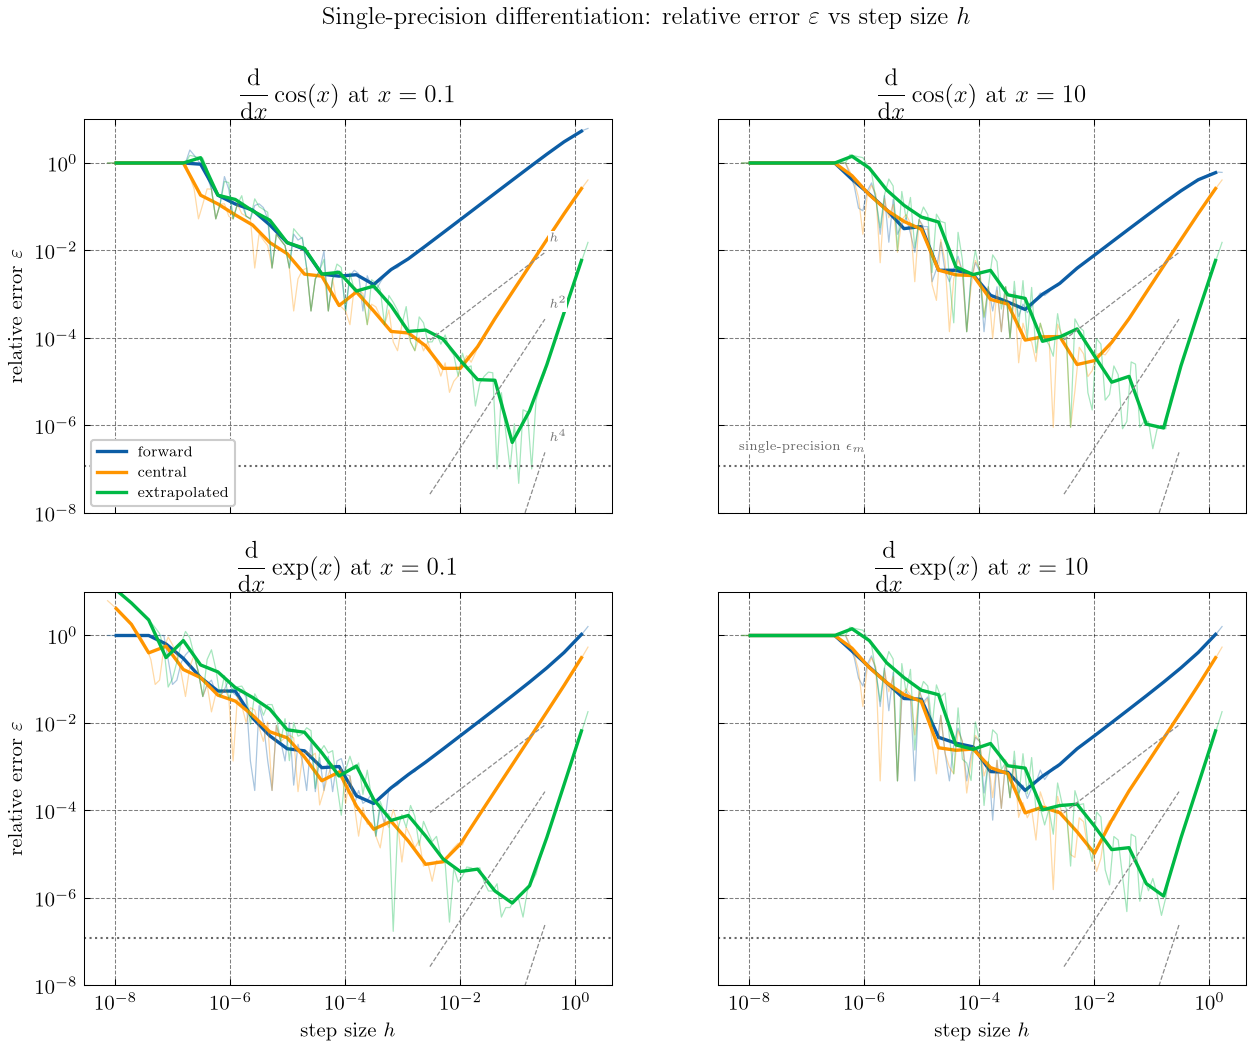
\includegraphics[width=\textwidth]{problem1_error.png}
\caption{Relative error $\eps$ of the single-precision forward (blue), central
(orange) and extrapolated (green) difference approximations to the derivative of
$\cos x$ (top) and $e^{x}$ (bottom) at $x=0.1$ (left) and $x=10$ (right), as a
function of the step size $h$. Thin lines are the raw results at 112 step sizes;
thick lines are the median in logarithmic bins in $h$. The dashed grey guides
have slopes $h$, $h^{2}$ and $h^{4}$, and the dotted horizontal line marks the
single-precision machine epsilon $\epsm=1.2\times10^{-7}$. For every method the
error decreases with the expected power of $h$ on the right (truncation regime),
passes through a minimum, and rises as $1/h$ with large scatter on the left
(round-off regime) until it saturates at $\eps=1$ where $f(x+h)$ and $f(x)$
become the same \code{float32} number.}
\label{fig:p1}
\end{figure}

Figure~\ref{fig:p1} shows the four cases. Table~\ref{tab:p1} compares the
simple estimates with what was measured; the measured columns give the range
over the four $(f,x)$ combinations.

\begin{table}[htbp]
\centering
\caption{Predicted and measured optimum step size and best relative error for
the three difference formulas in single precision. ``Trend'' rows refer to the
binned-median curves of Fig.~\ref{fig:p1}; ``raw best'' rows give the single
lowest raw point, which is systematically lower because it selects lucky
cancellations. Measured rows give the range over the four $(f,x)$ cases.}
\label{tab:p1}
\small
\begin{tabular}{llccc}
\toprule
method & & $h$ at minimum & $\eps_{\min}$ & digits\\
\midrule
forward, $O(h)$ & estimate & \sci{3.4}{-4} & \sci{3.4}{-4} & 3.5\\
 & trend & \sci{3}{-4}--\sci{6}{-4} & \sci{1.4}{-4}--\sci{1.7}{-3} & 2.8--3.8\\
 & raw best & \sci{2.6}{-5}--\sci{3.5}{-4} & \sci{2.6}{-5}--\sci{4.2}{-4} & 3.4--4.6\\
\midrule
central, $O(h^{2})$ & estimate & \sci{4.9}{-3} & \sci{2.4}{-5} & 4.6\\
 & trend & \sci{2.5}{-3}--\sci{1.0}{-2} & \sci{5.9}{-6}--\sci{2.5}{-5} & 4.6--5.2\\
 & raw best & \sci{2.0}{-3}--\sci{6.6}{-3} & \sci{9.1}{-7}--\sci{5.7}{-6} & 5.2--6.0\\
\midrule
extrapolated, $O(h^{4})$ & estimate & \sci{4.1}{-2} & \sci{2.9}{-6} & 5.5\\
 & trend & 0.08--0.16 & \sci{4.1}{-7}--\sci{1.1}{-6} & 6.0--6.4\\
 & raw best & \sci{6.9}{-4}--0.15 & \sci{4.8}{-8}--\sci{4.0}{-7} & 6.4--7.3\\
\bottomrule
\end{tabular}
\end{table}

\paragraph{Scaling and significant digits.}
On the large-$h$ side of each minimum the curves run parallel to the $h$,
$h^{2}$ and $h^{4}$ guides, confirming the order of each formula. The location
of the minimum moves to larger $h$ with increasing order, from a few times
$10^{-4}$ (forward) to a few times $10^{-3}$ (central) to $\sim0.1$
(extrapolated), in agreement with $h_{\mathrm{opt}}\sim\epsm^{1/(n+1)}$. The
extrapolated minimum sits a factor of 2--4 above the bare estimate because that
estimate drops prefactors: the leading truncation term of $D_{\mathrm{E}}$ is
$h^{4}f^{(5)}/480$, and balancing this small coefficient against the round-off
$\sim3\epsm/h$ of the three combined differences gives
$h_{\mathrm{opt}}\approx0.13$, inside the measured range. The error floors of
the trend curves give
roughly 3--4, 5 and 6 significant digits, bracketing the estimates of 3.5, 4.6
and 5.5. The spread within each method is the prefactor the estimate ignores:
the forward difference of $\cos x$ at $x=0.1$ is the worst case ($\eps$ floor
$1.7\times10^{-3}$) because $|f/f'| = \cot 0.1\approx10$ amplifies the
cancellation error tenfold, while $e^{x}$ with $|f/f'|=1$ reaches the estimate.
The extrapolated formula does slightly better than its estimate, and individual
raw points reach 7 digits for it, but this is the lucky-cancellation effect
rather than a systematic gain.

\paragraph{The truncation and round-off regimes.}
Three regimes are visible in every panel of Fig.~\ref{fig:p1}:
\begin{itemize}
\item \textbf{Large $h$ (right of the minimum): truncation.} The error is the
neglected Taylor term, so it is smooth, deterministic and falls as $h$, $h^{2}$
or $h^{4}$. The crossover to this regime moves to the right for higher order,
which is why the extrapolated formula is both the most accurate and the least
demanding on the choice of $h$.
\item \textbf{Small $h$ (left of the minimum): round-off.} $f(x+h)$ and $f(x)$
agree to more and more digits, the subtraction keeps only the disagreeing ones,
and the result is divided by $h$, so the error rises as $\epsm/h$, one decade
per decade. It is noisy because the cancellation error depends on the last bits
of the rounded function values, which change erratically with $h$. All three
formulas suffer equally here, since they differ only in how the same
cancelling differences are combined.
\item \textbf{Very small $h$: total loss.} For $h\lesssim2\times10^{-7}$ at
$x=0.1$ and $h\lesssim5\times10^{-7}$ at $x=10$ (where $x+h$ itself rounds back
to $x$), $f(x\pm h)$ is the same \code{float32} number as $f(x)$, the numerator
is exactly zero and the relative error saturates at $\eps=1$: the flat segments
at the far left.
\end{itemize}

\subsection*{Problem 2: quadrature}

\begin{figure}[htbp]
\centering
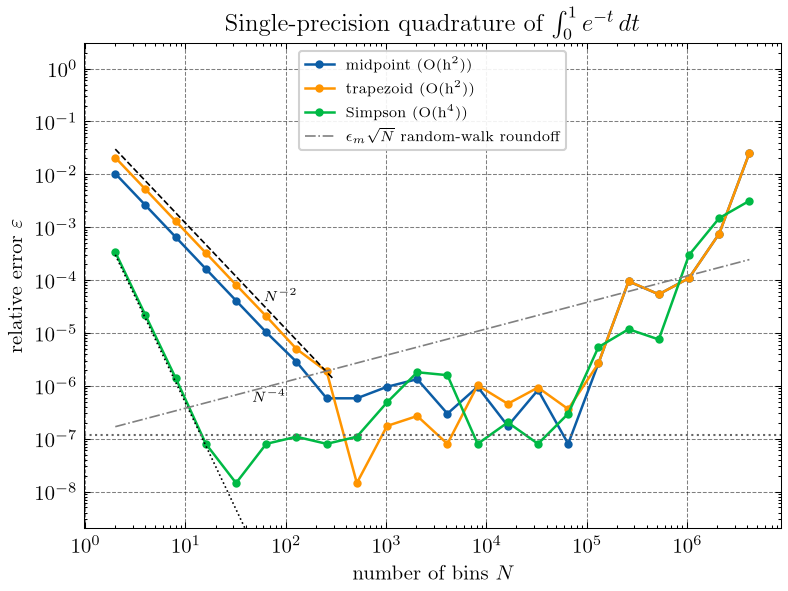
\includegraphics[width=0.8\textwidth]{problem2_error.png}
\caption{Relative error of the single-precision midpoint (blue), trapezoid
(orange) and Simpson (green) rules for $I=\int_0^1 e^{-t}\,dt$ as a function of
the number of bins $N=2^{1},\dots,2^{22}$. The dashed and dotted black lines are
$\propto N^{-2}$ and $N^{-4}$; the dash-dotted grey line is $\epsm\sqrt{N}$,
the random-walk estimate for accumulating $N$ rounding errors; the dotted
horizontal line is $\epsm$. The two second-order rules coincide in the
truncation regime and reach the $\sim10^{-7}$ floor near $N\approx300$, Simpson's
rule reaches it by $N\approx30$, and all three rise again past $N\sim10^{5}$,
more steeply than $\sqrt{N}$, because the \code{float32} running sum loses
precision as it grows.}
\label{fig:p2}
\end{figure}

Figure~\ref{fig:p2} shows three regimes.

\begin{itemize}
\item \textbf{Small $N$: truncation.} The midpoint and trapezoid errors fall as
$N^{-2}$ and lie almost on top of each other, as expected since their leading
error terms differ only by a factor of $-1/2$. Simpson's rule falls as $N^{-4}$
and is already at $10^{-7}$ by $N=32$. This regime is smooth and deterministic.
\item \textbf{Intermediate $N$: the single-precision floor.} Once the truncation
error drops below the precision of the accumulated sum, every rule flattens out
at $\eps\sim\epsm\approx10^{-7}$, about seven significant digits, and scatters
between $10^{-8}$ and $10^{-6}$ from one $N$ to the next. Simpson's rule hits the
floor at $N\approx30$, the second-order rules at $N\approx300$--$500$. Adding
bins beyond this point buys nothing.
\item \textbf{Large $N$: round-off growth.} Past $N\sim10^{5}$ the error rises
again, reaching $3\times10^{-3}$ to $2\times10^{-2}$ at $N=4\times10^{6}$, ten to
a hundred times above the $\epsm\sqrt{N}$ line. The nodes are exact for
power-of-two $N$, so this growth comes entirely from the running sum: the
accumulator grows to order $N$ while each term is of order one, so the rounding
error of each addition grows in proportion to the partial sum, and because the
integrand varies slowly, consecutive additions round almost identically: the
per-addition errors keep the same sign over runs of hundreds to $10^{6}$ terms
and add coherently rather than cancelling as a random walk. I confirmed this by
summing the identical
\code{float32} function values in double precision (or with pairwise summation
in \code{float32}), which keeps the error at $10^{-8}$ all the way to
$N=4\times10^{6}$.
\end{itemize}

The best accuracy is essentially the same for all three rules
(Table~\ref{tab:p2}), about seven to eight digits; the individual points below
$\epsm$ are fortunate roundings rather than a real gain. What distinguishes the
methods is the cost of getting there: Simpson's rule needs an order of magnitude
fewer function evaluations than the second-order rules.

\begin{table}[htbp]
\centering
\caption{Number of bins and relative error at the minimum of each curve in
Fig.~\ref{fig:p2}. The exact value is $I = 1-1/e = 0.6321205588$.}
\label{tab:p2}
\begin{tabular}{lccc}
\toprule
method & order & $N$ at minimum & minimum $\eps$\\
\midrule
midpoint  & $O(h^{2})$ & 65\,536 & \sci{8.0}{-8}\\
trapezoid & $O(h^{2})$ & 512     & \sci{1.5}{-8}\\
Simpson   & $O(h^{4})$ & 32      & \sci{1.5}{-8}\\
\bottomrule
\end{tabular}
\end{table}

\subsection*{Problem 3: the BAO peak}

\begin{figure}[htbp]
\centering
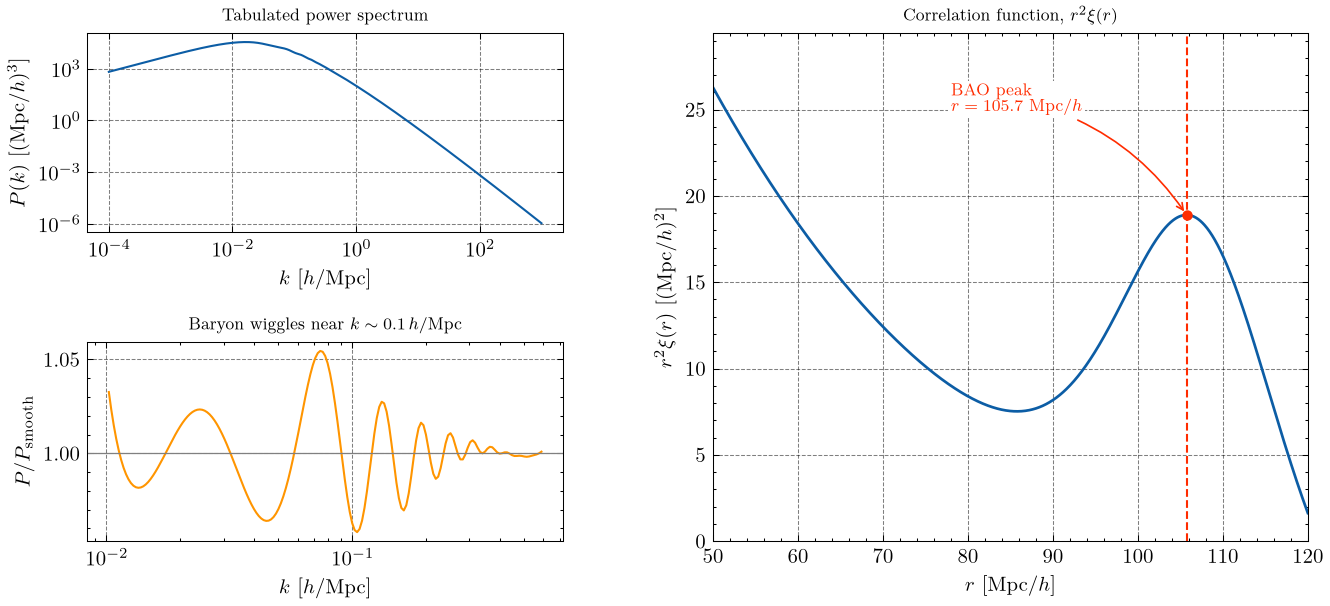
\includegraphics[width=\textwidth]{problem3_bao.png}
\caption{Left, top: the tabulated linear matter power spectrum $P(k)$ at $z=0$.
Left, bottom: $P(k)$ divided by a smooth sixth-order polynomial fit in
$\ln k$--$\ln P$ over $0.01<k<0.6\ h/\mathrm{Mpc}$, which exposes the baryon
wiggles, a damped oscillation of a few per cent amplitude around
$k\sim0.1\ h/\mathrm{Mpc}$. Right: the correlation function multiplied by
$r^{2}$ over $50\le r\le120\ \mathrm{Mpc}/h$, computed with
$k_{\max}=10\ h/\mathrm{Mpc}$, $\Delta k=2\times10^{-4}\ h/\mathrm{Mpc}$ and a
Gaussian taper at $k_d=3\ h/\mathrm{Mpc}$. The baryon wiggles in $k$ space
appear as a single bump in $r$ space; its maximum, the BAO peak, is marked by
the red point and dashed line at $r=105.7\ \mathrm{Mpc}/h$.}
\label{fig:p3}
\end{figure}

Figure~\ref{fig:p3} shows the input power spectrum, the baryon wiggles isolated
by dividing out a smooth fit, and the resulting $r^{2}\xi(r)$. The correlation
function decreases from $r^{2}\xi\approx26\ (\mathrm{Mpc}/h)^{2}$ at
$r=50\ \mathrm{Mpc}/h$ to a trough of $\approx7.5$ at
$r\approx86\ \mathrm{Mpc}/h$, rises to the BAO bump, and falls again toward
zero by $r=120\ \mathrm{Mpc}/h$.

\begin{table}[htbp]
\centering
\caption{Position of the BAO peak for different upper limits $k_{\max}$, $k$
steps and taper scales $k_d$ (``none'' is a hard cut at $k_{\max}$).}
\label{tab:p3}
\begin{tabular}{cccc}
\toprule
$k_{\max}$ [$h$/Mpc] & $\Delta k$ [$h$/Mpc] & $k_d$ [$h$/Mpc] & $r_{\mathrm{peak}}$ [Mpc/$h$]\\
\midrule
1  & \sci{2}{-4} & none & 103.77\\
2  & \sci{2}{-4} & none & 105.26\\
5  & \sci{2}{-4} & none & 106.18\\
10 & \sci{2}{-4} & none & 105.87\\
20 & \sci{2}{-4} & none & 105.71\\
10 & \sci{1}{-4} & 3 & 105.73\\
10 & \sci{5}{-4} & 3 & 105.73\\
10 & \sci{2}{-4} & 1 & 105.69\\
10 & \sci{2}{-4} & 3 & 105.73\\
20 & \sci{2}{-4} & 3 & 105.73\\
\bottomrule
\end{tabular}
\end{table}

\paragraph{Robustness of the upper limit.}
Table~\ref{tab:p3} lists the peak position for the tested settings. With a hard
cut, truncating at $k_{\max}=1\ h/\mathrm{Mpc}$ is visibly not converged (the
peak moves by $2\ \mathrm{Mpc}/h$), but for $k_{\max}\ge5\ h/\mathrm{Mpc}$ the
position is stable to better than $0.5\ \mathrm{Mpc}/h$, with the residual
wander caused by ringing of period $2\pi/k_{\max}$. Once the Gaussian taper is
applied, the result is identical to $0.01\ \mathrm{Mpc}/h$ whether
$k_{\max}=10$ or $20\ h/\mathrm{Mpc}$, whether $\Delta k$ is $10^{-4}$,
$2\times10^{-4}$ or $5\times10^{-4}\ h/\mathrm{Mpc}$, and changes by only
$0.04\ \mathrm{Mpc}/h$ if the taper is moved to $k_d=1\ h/\mathrm{Mpc}$. The
adopted setting, $k_{\max}=10\ h/\mathrm{Mpc}$ with $\Delta k=2\times10^{-4}$
and $k_d=3\ h/\mathrm{Mpc}$, is therefore converged.

\paragraph{Result.}
The BAO peak is at
\[
r_{\mathrm{peak}} = 105.7\ \mathrm{Mpc}/h,\qquad
r^{2}\xi(r_{\mathrm{peak}}) = 18.9\ (\mathrm{Mpc}/h)^{2},
\]
with a numerical uncertainty well below $0.5\ \mathrm{Mpc}/h$. This is the scale
of the sound horizon at the baryon-drag epoch imprinted in the matter
distribution, and it lies in the $\sim100$--$110\ \mathrm{Mpc}/h$ range expected
for a standard $\Lambda$CDM cosmology. The tabulated $\xi(r)$ is saved alongside
the code.

\section*{Code}

All code, the input power spectrum, the figures and the numerical outputs are in
the public GitHub repository
\begin{center}
\url{https://github.com/hz-xiaxz/compphys-hw1}
\end{center}
The scripts are plain Python (NumPy, SciPy, Matplotlib, SciencePlots) managed
with \code{uv}:
\begin{itemize}
\item \code{problem1.py}: forward, central and extrapolated differences in
single precision; writes \path{figs/problem1_error.png} and prints
Table~\ref{tab:p1}'s raw minima.
\item \code{problem2.py}: midpoint, trapezoid and Simpson rules with a naive
\code{float32} accumulator; writes \path{figs/problem2_error.png}.
\item \code{problem3.py}: log--log spline of $P(k)$, the split Simpson
integration, the convergence scan of Table~\ref{tab:p3}, the peak finder, and
\path{figs/problem3_bao.png}; also writes $\xi(r)$ to
\path{results/xi_of_r.txt}.
\item \code{plotstyle.py}: shared figure style. \code{results/} holds the
printed output of each script, and \code{writeup/} holds the source of this
document.
\end{itemize}
Running \code{uv sync} followed by \code{uv run python problemN.py} reproduces
every figure and number quoted here.

\end{document}
